\documentclass[a4paper,12pt]{article}
\usepackage[bahasa]{babel}
\usepackage{graphicx}
\usepackage{multirow}
\usepackage{enumitem}
\usepackage{listings}
\graphicspath{ {./img/} }
\begin{document}
\title{Laporan Praktikum Statistika Pertemuan 9}
%\author{Aldzikri Dwijayanto Prathama \\ {\small 195410189}}
\author{Aldzikri Dwijayanto Prathama 
	\\195410189}
\makeatletter
\begin{titlepage}
	\begin{center}
		{\huge \bfseries \@title }\\[14ex]
		
\includegraphics[scale=.8]{logo}\\[4ex]
		{\large \@author}\\[20ex]
		{\large \bfseries {SEKOLAH TINGGI MANAJEMEN INFORMATIKA DAN KOMPUTER
				AKAKOM YOGYAKARTA}}
	\end{center}


%{\large \@date} 
\end{titlepage}
\makeatother
%\maketitle
\newpage
\tableofcontents
\newpage
\section{Pembahasan}
\subsection{Praktik}
\subsubsection{Praktik 1}
\paragraph{}
Pada praktik pertama dilakukan penghitungan terhadap keuntungan bersih pertahun dari 50 perusahaan batik di Yogyakarta, datanya adalah sebagai berikut: 60 33 85 52 65 77 84 65 57 77 71 81 35 50 38 64 74 41 68 54 41 41 61 91 55 73 54 53 45 77
\begin{center}
	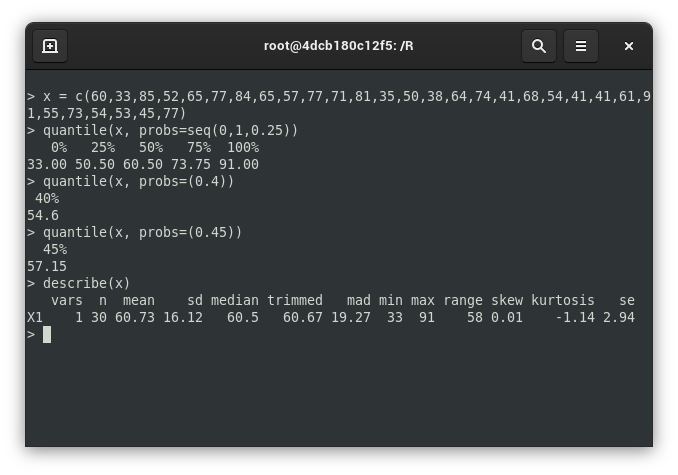
\includegraphics[scale=.5]{1}
\end{center}
\begin{enumerate}[label=\alph*.]
	\item Kuartil merupakan ukuran letak yang membagi data yang sudah diurutkan menjadi empat bagian sama banyak, masing-masing bagian mempunyai 25\% data.
	Kelompok data memiliki 3 kuartil yakni kuartil bawah (Q$_{1}$), kuartil tengah atau median (Q$_{2}$), Quartil atas (Q$_{3}$). 
	\\Untuk menentukan Q$_{1}$, Q$_{2}$, dan Q$_{3}$ dari data keuntungan bersih perusahaan batik di Yogyakarta, pertama-tama masukkan data ke dalam variabel terlebih dahulu\\
	\texttt{x = c(60,33,85,52,65,77,84,65,57,77,71,81,35,50,38,64,74\\,41,68,54,41,41,61,91,55,73,54,53,45,77)\\}
	Setelah data dimasukkan ke variabel x, tentukan kuartil dengan fungsi quantile\\
	\texttt{quantile(x, probs=seq(0,1,0.25))\\}
	kuartil terletak di 25\%, 50\%, dan 75\% dari data, itu berarti nilai Q$_{1}$ nya adalah 50,50 , Q$_{2}$nya adalah 60,50, sedangkan Q$_{3}$nya adalah 73,75
	
	\item Desil merupakan  ukuran letak yang membagi data yang sudah diurutkan dari terkecil hingga terbesar menjadi sepuluh bagian sama banyak. Jadi masing-masing bagian memiliki 10 \% data keseluruhan dan memiliki 9 nilai desil.\\
	untuk menentukan D$_{4}$ dari data keuntungan bersih perusahaan batik di Yogyakarta, masukkan data ke dalam variabel terlebih dahulu\\
	\texttt{x = c(60,33,85,52,65,77,84,65,57,77,71,81,35,50,38,64,74\\,41,68,54,41,41,61,91,55,73,54,53,45,77)\\}
	Setelah data dimasukkan ke variabel x, tentukan desil dengan fungsi quantile, karena masing-masing bagian desil memiliki 10\% data keselurahan maka D$_{4}$ = 10\% * 4, maka nilai di probs adalah 0.4 maka digunakan perintah\\
	\texttt{quantile(x, probs=seq(0,4))\\}
	dari outpuynya terlihat bahwa D$_{4}$ memiliki nilai 54,6
\end{enumerate}


\end{document}